\chapter{Ciò che lega cambiamento climatico e inflazione}
\label{chp2}

\section{Il mandato BCE}

In Europa, l'analisi del fenomeno inflattivo non può prescindere dal ruolo ricoperto dalla Banca Centrale Europea. Insieme al Sistema Europeo delle Banche Centrali (SEBC) di cui fa parte, l'\textit{European Cental Bank} è istituita con il Trattato di Maastricht nel 1992 e costituita il 1° giugno 1998 con lo Statuto del Sistema Europeo di Banche Centrali e della Banca Centrale Europea. Oggi, la Banca Centrale Europea fa parte integrante del quadro istituzionale dell'Unione Europea grazie all'\mbox{articolo 13} del Trattato sull'Unione Europea. Le competenze e gli obiettivi principali della BCE sono espressi, in particolare, nei seguenti due articoli dei Trattati:

\begin{displayquote}
	\small\singlespacing{Art. 3 c. 3, TUE\\}\textit{
		L'Unione instaura un mercato interno. Si adopera per lo sviluppo sostenibile dell'Europa, basato su una crescita economica equilibrata e sulla stabilità dei prezzi, su un'economia sociale di mercato fortemente competitiva, che mira alla piena occupazione e al progresso sociale, e su un elevato livello di tutela e di miglioramento della qualità dell'ambiente. [...]}
	\small\singlespacing{Art. 127 c. 1, TFUE\\}\textit{
		L'obiettivo principale del Sistema europeo di banche centrali, in appresso denominato «SEBC», è il mantenimento della stabilità dei prezzi. Fatto salvo l'obiettivo della stabilità dei prezzi, il SEBC	sostiene le politiche economiche generali nell'Unione al fine di contribuire alla realizzazione degli obiettivi dell'Unione definiti nell'articolo 3 del trattato sull'Unione europea. [...]}
\end{displayquote}

Il mantenimento della stabilità dei prezzi, ossia il controllo dell'inflazione, è il mandato primario dell'ECB. Questa volontà degli Stati, espressa all'interno dei Trattati, mette in luce l'influenza che i prezzi hanno sulla vita delle persone e la vicinanza che si è voluta dare alle istituzioni europee che si mettono quotidianamente al servizio dei cittadini dell'Unione.

Nel definire la politica monetaria per l'area Euro, la Banca centrale identifica e comunica al pubblico gli obiettivi che intende raggiungere, così come gli strumenti convenzionali che impiegherà durante il suo mandato. Questo tipo di comunicazioni sono fondamentali per garantire la trasparenza, l'indipendenza e la credibilità del suo operato, oltre che ancorare le aspettative degli operatori di mercato ai target prefissati. Negli anni, gli elementi che compongono la strategia di politica monetaria sono profondamente cambiati. Negli anni Settanta e Ottanta, molte banche centrali, come la \textit{Deutsche Bundesbank} o la Banca d'Italia, fissavano target di crescita degli aggregati monetari M2 o M3 per il controllo dell'inflazione \parencite{DB:monetary_policy_strategies}. Questo strumento di analisi dell'andamento economico è stato ereditato anche dalla BCE e utilizzato attivamente sino alle crisi economico finanziarie dei primi anni Duemila. Gli avvenimenti dirompenti di inizio secolo hanno evidenziato la necessità di nuovi meccanismi di ascolto e, con la recente \textit{monetary policy strategy review} pubblicata l'8 luglio 2021, la \textit{two-pillar strategy} è stata ufficialmente abbandonata. In precedenza, le decisioni del \textit{Governing Council} ECB venivano prese confrontando le informazioni provenienti da due distinti pilastri, uno economico e l'altro monetario e finanziario, oggi la Banca centrale si impegna a sviluppare e utilizzare un modello decisionale integrato \parencite{ECB:overview_strategy_review}.

Più in dettaglio, il mandato primario della BCE si traduce nell'operare affinché l'inflazione assuma un valore tendente al 2\% nel medio periodo. Questa strategia prende il nome di \textit{inflation targeting} e l'indice utilizzato per misurare la variazione dei prezzi è il già citato \textit{Harmonised Index of Consumer Prices} (HICP) riportato in Figura \ref{img:inflation_ea_2022}. Con la recente revisione della politica monetaria, questo obiettivo quantitativo è simmetrico attorno al 2\%, con la novità quindi, di considerare indesiderata anche un'eccessiva deflazione. In passato, la \textit{monetary strategy} europea ha avuto target d'inflazione differenti: nel 1998 si fissava il \textit{cap} al 2\%, mentre nel 2003 si accettavano anche valori prossimi al 2\%. Un'inflazione obiettivo al 2\% è da alcuni considerata troppo bassa e l'articolo \textit{"Rethinking the ECB's inflation objective"} di Ethan Ilzetzki pubblicato sul sito VoxEU.org condivide alcune considerazioni  \parencite{Ilzetzki:inflation_target}. Ilzetzki riporta i risultati di un sondaggio fra gli economisti del \textit{Centre for Macroeconomics}: la maggior parte di loro risulta essere favorevole ad un'inflazione che eccede il 2\% in seguito a periodi con bassa inflazione; e circa il 30\% di loro sosterrebbe un aumento del tasso target di inflazione oltre l'attuale 2\%. Il principale strumento di politica monetaria in mano alle Banche centrali sono i tassi d'interesse a breve termine (\textit{overnight}) applicati alle riserve del mercato interbancario. Il loro livello influenza direttamente l'operato delle banche e indirettamente il sistema economico. La Figura \ref{img:interest_rate_transmission} sottostante mostra il meccanismo di trasmissione della politica monetaria a partire dai tassi del mercato monetario.

\begin{figure}[h]
	\centering
	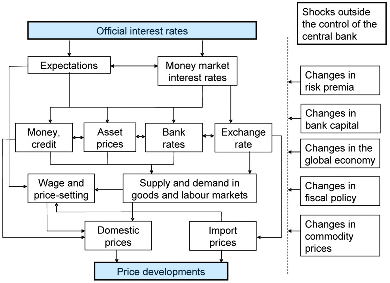
\includegraphics[width=0.80\textwidth]{img/interest_rates_transmission.pdf}
	\caption{}
	\source{\cite{ECB:transmission_mechanism}}
	\label{img:interest_rate_transmission}
\end{figure}

I promotori di un tasso inflazionistico obiettivo superiore all'attuale, ossia nell'ordine del 3-5\%, sostengono che ciò allontanerebbe il ripresentarsi di tassi d'interesse pari o prossimi allo zero. Se prima delle crisi di inizio secolo lo \textit{zero lower bound} era esistito solamente sui libri di testo, da un decennio a questa parte è realtà. Ciò significa che i tassi a breve termine applicati dalle Banche centrali sono pari a zero, se non negativi. A dimostrazione di ciò, la Tabella \ref{table:tassi_ecb} riporta i tassi applicati dalla Banca Centrale Europea negli ultimi anni ad oggi:

\begin{table}[h]
	\centering
	\begin{tabularx}{.8\textwidth}{@{}llll@{}}
		\toprule
		& \textbf{MRO}   & \textbf{deposit facility} & \textbf{marginal lending facility} \\ \midrule
		2019 & -0,50 & 0,00 & 0,25 \\
		2016 & -0,40 & 0,00 & 0,25 \\
		2015 & -0,30 & 0,05 & 0,30 \\ \bottomrule
	\end{tabularx}
	\caption{}
	\source{\cite{ECB:key_interest_rates}}
	\label{table:tassi_ecb}
\end{table}

La situazione che si genera è chiamata "trappola della liquidità", poiché le decisioni di politica monetaria perdono di efficacia nei confronti dell'economia reale. L'Equazione \ref{formula:interesse_inflazione} descrive il legame tra tasso nominale ($i$), tasso reale ($r$) e inflazione ($\pi$):

\begin{equation}
	\label{formula:interesse_inflazione}
	i = r + \pi
\end{equation}

Le Banche centrali fissano il tasso nominale $i$, gli agenti economici sono condizionati dal tasso reale $r$ e l'inflazione $\pi$ è data. In presenza di una recessione, un'inflazione sostenuta permette di ridurre maggiormente il tasso reale, pur rispettando il limite inferire dello 0\% del tasso nominale. Ciò non può avvenire in presenza di bassa inflazione, non potendo così stimolare l'economia reale quanto si vorrebbe.

Tutti questi elementi a sostegno di un'inflazione più sostenuta però, trovano come inderogabile limite il mandato primario perseguito dalla Banca Centrale Europea: la stabilità dei prezzi.

\section{Politica monetaria e climateflation}

Il cambiamento climatico è una delle più complesse sfide che l'umanità sta affrontando. Da qualche anno a questa parte, stiamo assistendo a governi, organizzazioni e società civile intraprendere azioni e decisioni per mitigare gli effetti di questo evento e diventare una società sempre meno dipendente dalle fonti energetiche fossili. I governi e i parlamenti nazionali hanno la responsabilità primaria di impegnarsi in questa transizione verso un mondo più sostenibile. Inizialmente, potremmo credere che le banche centrali non giochino alcun ruolo in questa sfida globale, ma così non è. Anche la politica monetaria è influenzata dal \textit{climate change} e cinque sono i canali attraverso cui viene colpita \parencite{ECB:to_be_green}.

\begin{figure}[h]
	\centering
	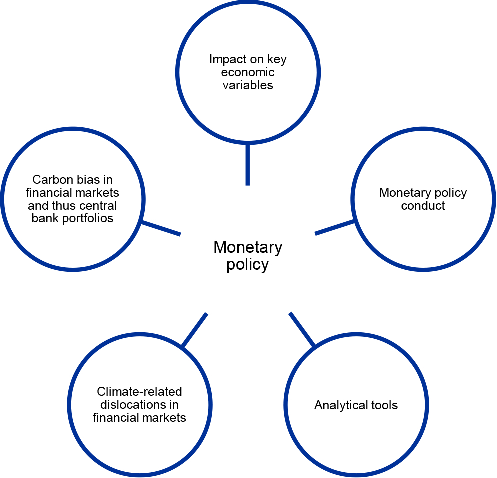
\includegraphics[width=0.80\textwidth]{img/monetary_policy_circle.pdf}
	\caption{}
	\source{\cite{ECB:to_be_green}}
	\label{img:monetary_policy_circle}
\end{figure}

\begin{enumerate}
\item Un cambiamento climatico non gestito può degenerare e rendere più frequenti gli eventi climatici estremi e distruttivi, con conseguenti e continui shock sull'economia. Dal lato dell'offerta, un evento estremo aumenta i costi di produzione, e quindi i prezzi, oltre che ridurre l'output. La domanda, soprattutto per gli investimenti, si riduce a causa della maggiore incertezza. L'impatto sulle variabili macroeconomiche, come prezzi, produzione e lavoro, è evidente.

\item La conduzione della politica monetaria diventa più difficoltosa a causa della maggiore volatilità dei prezzi e la crescente incertezza.

\item Il cambiamento climatico provoca shock sempre più persistenti con effetti di medio e lungo periodo. L'analisi economica e gli strumenti di ascolto e previsione delle banche centrali devono evolversi ed estendere il loro raggio d'azione.

\item Rivalutare il rischio climatico a cui sono esposte le attività finanziarie e la~generale transizione verso un'economia e mercati finanziari \textit{low-carbon}, può generare shock finanziari ed economici che la politica monetaria deve~considerare.

\item All'interno del programma di quantitative easing europeo \textit{"Corporate Sector Purchase Programme"} (CSPP), la Banca centrale ha acquistato massivamente titoli emessi da numerose aziende, rendendosi però protagonista di un \textit{"carbon bias"}. Il report \textit{"Decarbonising is easy: beyond market neutrality in the ECB's corporate QE"} pubblicato dal think tank New Economics Foundation mostra l'elevato coinvolgimento della BCE in aziende \textit{carbon-intensive} \parencite{NEF:carbon_bias_report}. Il 62,7\% del portafoglio BCE è riconducibile a settori ad elevata emissione di carbonio, responsabili di circa il 58,5\% delle emissioni di gas serra in Europa e che formano solo il 18\% del valore aggiunto europeo. Nell'ottica di una transizione anche finanziaria, comunque proteggendo il bilancio BCE, la politica monetaria deve rivedere e controllare maggiormente il proprio portafoglio.
\end{enumerate}

Oggi, la Banca Centrale Europea riconosce pienamente la rilevanza e il possibile impatto di questi rischi e quindi si impegna, nell'ambito del suo mandato, a contrastare gli effetti indesiderati del cambiamento climatico. Questo nuovo obiettivo operativo, se non altro come principio guida, è un'assoluta novità. Recita così la nuova \textit{monetary policy strategy review} presentata nel luglio 2021:

\begin{displayquote}
	\small\singlespacing\textit{The Governing Council is committed – within the ECB’s mandate – to ensuring that the Eurosystem fully takes into account the implications of climate change and the carbon transition for monetary policy and central banking.} \parencite{ECB:overview_strategy_review}
\end{displayquote}

Questo nuovo elemento fondamentale della politica monetaria, quasi un "nuovo pilastro", si è già tradotto nella realizzazione di una roadmap ambiziosa che la BCE intende seguire, di cui viene mostrato un estratto in Figura \ref{ECB:roadmap_inflation}, e nella costituzione di un \textit{"Climate Change Center"} all'interno della Banca centrale.

\begin{figure}[h]
	\centering
	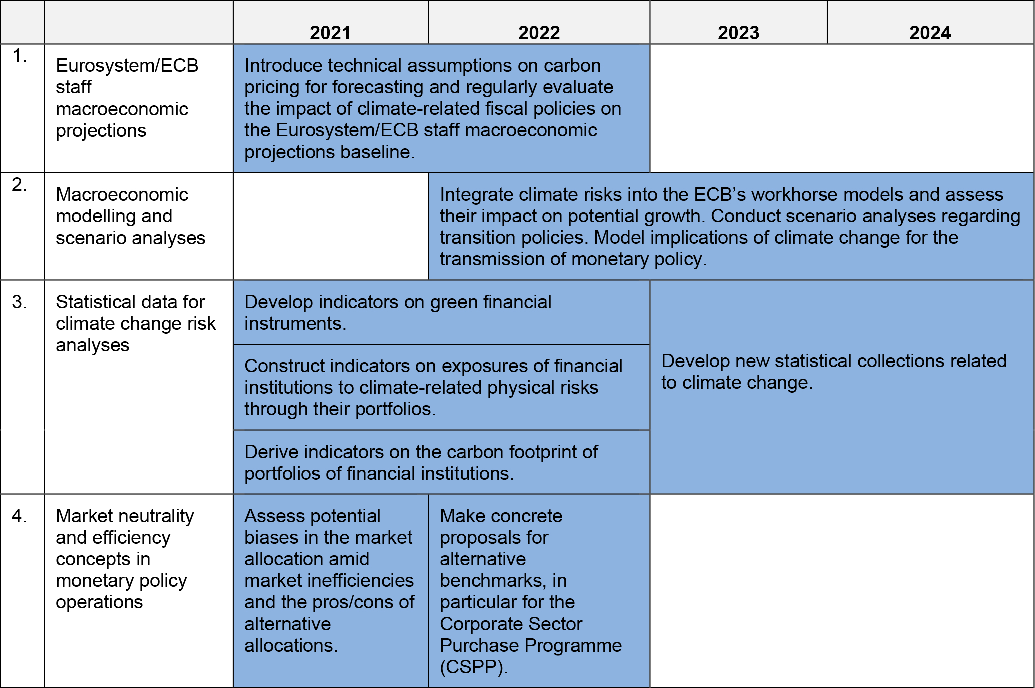
\includegraphics[width=0.80\textwidth]{img/inflation_roadmap.pdf}
	\caption{}
	\source{\cite{ECB:inflation_roadmap}}
	\label{ECB:roadmap_inflation}
\end{figure}

Col passare del tempo, sono sempre più evidenti gli sforzi della BCE per cercare di internalizzare il cambiamento climatico nella sua \textit{policy strategy}. Un recente discorso di Isabel Schnabel, uno dei sei membri del Comitato esecutivo della Banca centrale, tenuto il 17 marzo 2022, ha ulteriormente formalizzato la necessità di rendersi indipendenti dalle fonti energetiche fossili \parencite{ECB:speech_isabel}. Il petrolio è una fonte energetica che non solo mina la sopravvivenza sul nostro pianeta, ma come la situazione geopolitica ci sta insegnando, mette a rischio anche i nostri valori, la nostra libertà e democrazia. Per questo, le fonti energetiche rinnovabili non sono solo sostenibili, sono anche \textit{"freedom energies"}. Schnabel continua sostenendo che questa transizione energetica verde presenta un costo che vale la pena pagare. Siamo di fronte a un'era caratterizzata da un'inflazione generata dal cambiamento climatico e dalle fonti energetiche, che probabilmente sarà persistente nel tempo, e che possiamo scomporre in tre componenti.

\begin{enumerate}

\item \textit{Climateflation}. Il costo del cambiamento climatico stesso. La frequenza di eventi atmosferici estremi è in aumento e così il loro impatto sull'attività umana e sull'economia. Ad esempio, lunghi periodi di siccità stanno già causando problemi alla catena alimentare, con conseguenti aumenti nei prezzi del cibo.

\item \textit{Fossilflation}. Nel 2019, l'85\% dell'energia usata in Europa derivava da petrolio e gas naturale. Negli ultimi mesi, abbiamo sperimentato le conseguenze economiche della nostra dipendenza da queste fonti energetiche. L'aumento dei prezzi è stato causato dall'incertezza geopolitica e dalle speculazioni, ma la stessa lotta al cambiamento climatico è un fattore che rende più costosi i derivati fossili.

\item \textit{Greenflation}. La transizione verde ha un costo per le aziende. I nuovi costi per adattare e innovare gli impianti o i processi produttivi, con l'obiettivo di ridurre le emissioni di carbonio, non possono essere per intero assorbiti dalle imprese e devono quindi essere trasferiti al pubblico. Inoltre, l'aumento simultaneo e generalizzato della domanda di una serie di prodotti, come minerali, metalli o pannelli solari, almeno nel breve e medio termine, si traduce in un'offerta incapace di soddisfare la domanda.

\end{enumerate}

Concludendo il suo discorso, Schnabel rimarca il ruolo centrale della BCE in questo periodo di transizione. Non solo per indirizzare e finanziare il cambiamento verso le tecnologie più promettenti, ma soprattutto, ricordando il mandato primario conferito dai Trattati, per difendere il potere di acquisto delle persone.

\begin{displayquote}
	\small\singlespacing\textit{Monetary policy will play its role in this transition. It will protect the purchasing power of people by ensuring that the current protracted period of high inflation will not become entrenched in expectations, while remaining supportive of growth and employment.}\\ \parencite{ECB:speech_isabel}
\end{displayquote}
















